\section*{1. Berechnung der Hypotenuse}
Berechne die Länge der Hypotenuse in den folgenden rechtwinkligen Dreiecken:
\begin{enumerate}
    \item $a = 7$ cm, $b = 24$ cm
    \begin{center}
    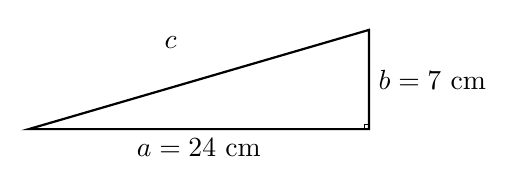
\begin{tikzpicture}[scale=0.18]
      \draw[thick] (0,0) -- (24,0) -- (24,7) -- cycle;
      \draw (12,0) node[below]{$a=24$ cm};
      \draw (24,3.5) node[right]{$b=7$ cm};
      \draw (10,4) node[above, yshift=5pt]{$c$};
      \draw (24,0) rectangle (23.7,0.3);
    \end{tikzpicture}
    \end{center}
    \item $a = 9{,}5$ cm, $b = 12{,}2$ cm
    \begin{center}
    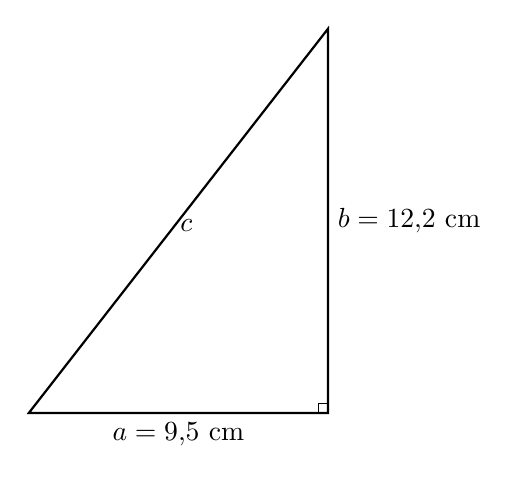
\begin{tikzpicture}[scale=0.4]
      \draw[thick] (0,0) -- (9.5,0) -- (9.5,12.2) -- cycle;
      \draw (4.75,0) node[below]{$a=9{,}5$ cm};
      \draw (9.5,6.1) node[right]{$b=12{,}2$ cm};
      \draw (5,5) node[above, yshift=5pt]{$c$};
      \draw (9.5,0) rectangle (9.2,0.3);
    \end{tikzpicture}
    \end{center}
    \item $a = 15$ cm, $b = 20$ cm
    \begin{center}
    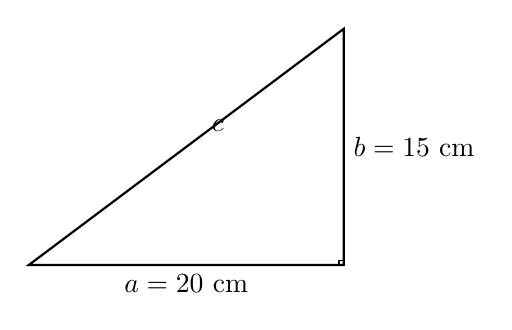
\begin{tikzpicture}[scale=0.2]
      \draw[thick] (0,0) -- (20,0) -- (20,15) -- cycle;
      \draw (10,0) node[below]{$a=20$ cm};
      \draw (20,7.5) node[right]{$b=15$ cm};
      \draw (12,7) node[above, yshift=5pt]{$c$};
      \draw (20,0) rectangle (19.7,0.3);
    \end{tikzpicture}
    \end{center}
\end{enumerate}

\section*{2. Berechnung einer Kathete}
Bestimme die fehlende Kathete:
\begin{enumerate}
    \item $c = 13$ cm, $a = 5$ cm
    \begin{center}
    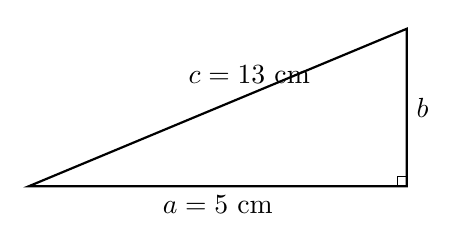
\begin{tikzpicture}[scale=0.4]
      \draw[thick] (0,0) -- (12,0) -- (12,5) -- cycle;
      \draw (6,0) node[below]{$a=5$ cm};
      \draw (12,2.5) node[right]{$b$};
      \draw (7,2.5) node[above, yshift=5pt]{$c=13$ cm};
      \draw (12,0) rectangle (11.7,0.3);
    \end{tikzpicture}
    \end{center}
    \item $c = 25$ cm, $a = 7$ cm
    \begin{center}
    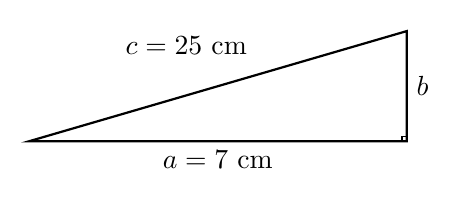
\begin{tikzpicture}[scale=0.2]
      \draw[thick] (0,0) -- (24,0) -- (24,7) -- cycle;
      \draw (12,0) node[below]{$a=7$ cm};
      \draw (24,3.5) node[right]{$b$};
      \draw (10,4) node[above, yshift=5pt]{$c=25$ cm};
      \draw (24,0) rectangle (23.7,0.3);
    \end{tikzpicture}
    \end{center}
    \item $c = 10$ cm, $b = 6$ cm
    \begin{center}
    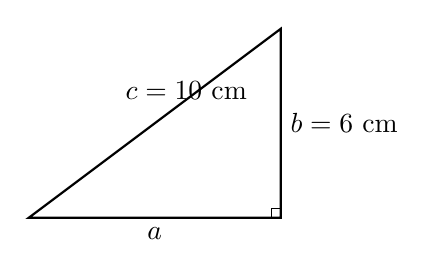
\begin{tikzpicture}[scale=0.4]
      \draw[thick] (0,0) -- (8,0) -- (8,6) -- cycle;
      \draw (4,0) node[below]{$a$};
      \draw (8,3) node[right]{$b=6$ cm};
      \draw (5,3) node[above, yshift=5pt]{$c=10$ cm};
      \draw (8,0) rectangle (7.7,0.3);
    \end{tikzpicture}
    \end{center}
\end{enumerate}

\section*{3. Höhenberechnung}
Ein Baum wirft einen 9 m langen Schatten. Der Einfallswinkel der Sonne beträgt 60°.  
Berechne die Höhe des Baumes unter der Annahme, dass der Schatten auf ebenem Boden liegt.

\begin{center}
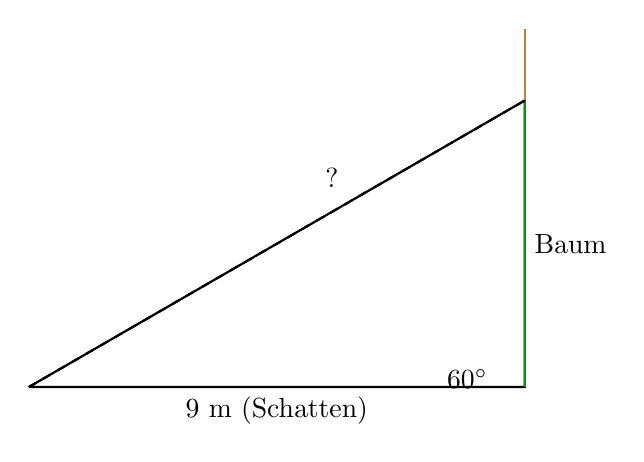
\begin{tikzpicture}[scale=0.7]
  \draw[thick] (0,0) -- (9,0) -- (9,5.2) -- (0,0);
  \draw[thick, green!60!black] (9,0) -- (9,5.2);
  \draw[thick, brown] (9,5.2) -- (9,6.5);
  \draw[thick, dashed] (0,0) -- (9,5.2);
  \draw (4.5,0) node[below]{9 m (Schatten)};
  \draw (9,2.6) node[right]{Baum};
  \draw (5.5,3.2) node[above, yshift=5pt]{?};
  \draw (8.5,0.5) node[below left]{60$^\circ$};
\end{tikzpicture}
\end{center}

\section*{4. Dreieck auf einem Dach}
Ein Satteldach hat eine Dachneigung von 40° und eine Breite von 6 m. Berechne die Länge der Dachflächen.

\begin{center}
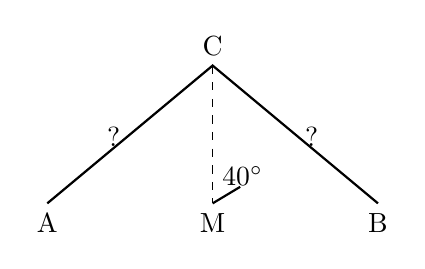
\begin{tikzpicture}[scale=0.7]
  \draw[thick] (0,0) -- (3,2.5) -- (6,0);
  \draw[dashed] (3,2.5) -- (3,0);
  \draw (0,0) node[below]{A};
  \draw (6,0) node[below]{B};
  \draw (3,2.5) node[above]{C};
  \draw (3,0) node[below]{M};
  \draw (1.5,1.2) node[left]{?};
  \draw (4.5,1.2) node[right]{?};
  \draw (3,0.5) node[right]{40$^\circ$};
  \draw[thick] (3,0) -- (3.5,0.3);
\end{tikzpicture}
\end{center}

\section*{5. Diagonale in einem Quader}
Ein Quader hat die Kantenlängen 3 cm, 4 cm und 12 cm.
\begin{enumerate}
    \item Berechne die Raumdiagonale.
    \begin{center}
    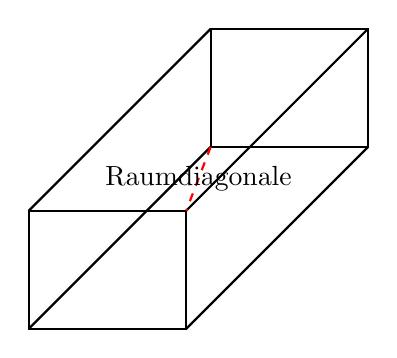
\begin{tikzpicture}[scale=0.5]
      \draw[thick] (0,0,0) -- (4,0,0) -- (4,3,0) -- (0,3,0) -- cycle;
      \draw[thick] (0,0,0) -- (0,0,12);
      \draw[thick] (4,0,0) -- (4,0,12);
      \draw[thick] (4,3,0) -- (4,3,12);
      \draw[thick] (0,3,0) -- (0,3,12);
      \draw[thick] (0,0,12) -- (4,0,12) -- (4,3,12) -- (0,3,12) -- cycle;
      \draw[thick, dashed, red] (0,0,0) -- (4,3,12);
      \node at (2,1.5,6) {Raumdiagonale};
    \end{tikzpicture}
    \end{center}
    \item Berechne die Länge der Diagonalen der Grundfläche.
    \begin{center}
    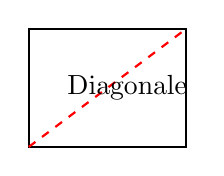
\begin{tikzpicture}[scale=0.5]
      \draw[thick] (0,0) -- (4,0) -- (4,3) -- (0,3) -- cycle;
      \draw[thick, dashed, red] (0,0) -- (4,3);
      \node at (2.5,1.5) {Diagonale};
    \end{tikzpicture}
    \end{center}
\end{enumerate}

\section*{6. Anwendung auf eine Leiter}
Eine 5 m lange Leiter lehnt an einer Wand. Der Fuß der Leiter ist 1,5 m von der Wand entfernt.  
\begin{enumerate}
    \item Wie hoch reicht die Leiter an der Wand?  
    \begin{center}
    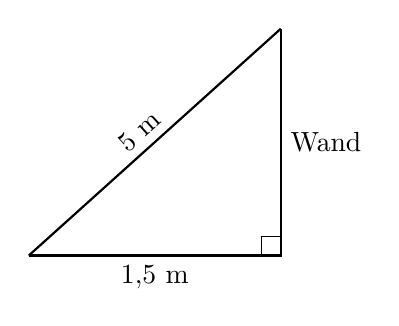
\begin{tikzpicture}[scale=0.8]
      \draw[thick] (0,0) -- (4,0) -- (4,3.6);
      \draw[thick] (0,0) -- (4,3.6);
      \draw (2,0) node[below]{$1{,}5$ m};
      \draw (4,1.8) node[right]{Wand};
      \draw (2.2,1.8) node[above, rotate=42, xshift=-5pt, yshift=3pt]{$5$ m};
      \draw (4,0) rectangle (3.7,0.3);
    \end{tikzpicture}
    \end{center}
    \item Falls die Leiter um 0,5 m nach hinten gezogen wird, wie hoch reicht sie dann?  
    \begin{center}
    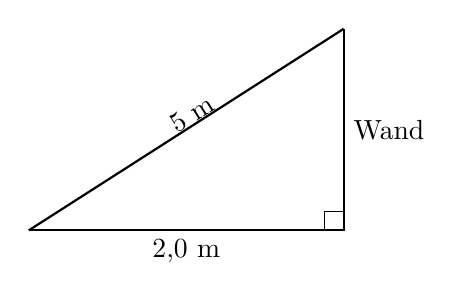
\begin{tikzpicture}[scale=0.8]
      \draw[thick] (0,0) -- (5,0) -- (5,3.2);
      \draw[thick] (0,0) -- (5,3.2);
      \draw (2.5,0) node[below]{$2{,}0$ m};
      \draw (5,1.6) node[right]{Wand};
      \draw (3,1.6) node[above, rotate=32, xshift=-5pt, yshift=3pt]{$5$ m};
      \draw (5,0) rectangle (4.7,0.3);
    \end{tikzpicture}
    \end{center}
\end{enumerate}

\section*{7. Herausforderung: Dreieck in einem Kreis}
Ein Kreis hat den Durchmesser 10 cm. Ein rechtwinkliges Dreieck wird so in den Kreis gezeichnet, dass die Hypotenuse dem Durchmesser entspricht. Berechne die möglichen Kathetenlängen, wenn eine Kathete 6 cm lang ist.

\begin{center}
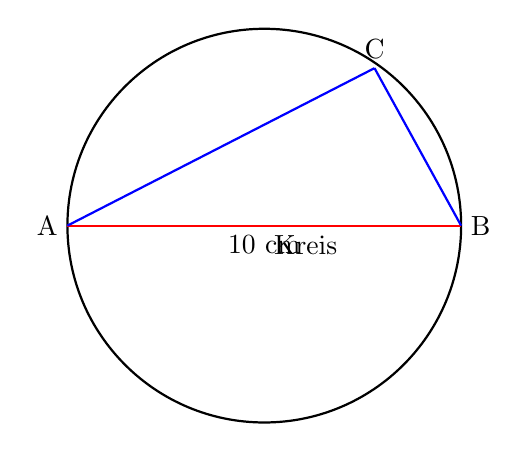
\begin{tikzpicture}[scale=0.5]
  \draw[thick] (0,0) circle(5);
  \draw[thick, red] (-5,0) -- (5,0);
  \draw[thick, blue] (-5,0) -- (2.8,4.0);
  \draw[thick, blue] (2.8,4.0) -- (5,0);
  \node[below] at (0,0) {10 cm};
  \node[left] at (-5,0) {A};
  \node[right] at (5,0) {B};
  \node[above] at (2.8,4.0) {C};
  \draw (0,0) node[below right]{Kreis};
\end{tikzpicture}
\end{center}
